\subsection{MOOSE}
\begin{frame}
\frametitle{MOOSE}
\begin{columns}
    \column[t]{4cm}
	\begin{itemize}
    	\item Computational framework
    	\item Solves coupled equation systems
    	\item MOOSE defines weak forms
    	\item MOOSE and LibMesh translate them into residual and Jacobian functions
    	\item PetSc solution routines solve the equations
    \end{itemize}

	\column[t]{6cm}
	\begin{figure}[htbp!]
		\begin{center}
			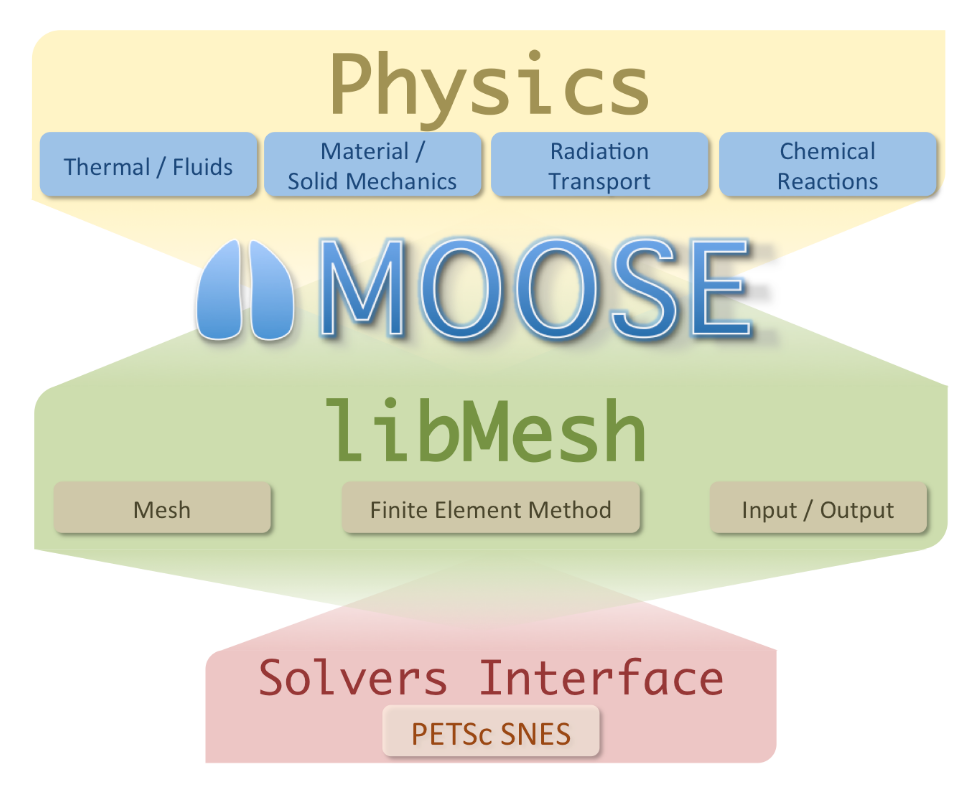
\includegraphics[width=6cm]{moose}
		\end{center}
		\caption{MOOSE framework. Image reproduced from \cite{inl_workshop_2020}.}
	\end{figure}
\end{columns}
\end{frame}


\subsection{$SP_3$}
\begin{frame}
\frametitle{$P_3$ equations}

\begin{align}
    & \frac{d}{dx} \phi_{1,g} + \Sigma_{t,g} \phi_{0,g} = \sum_{g'=1}^G \Sigma_{s0,g' \rightarrow g} \phi_{0,g'} + \frac{\chi_g}{k_{eff}} \sum_{g'=1}^G \nu\Sigma_{f,g'} \phi_{0,g'} + Q_{0,g}  \label{eq:SP3-0} \\
    & \frac{1}{3} \frac{d}{dx} \phi_{0,g} + \frac{2}{3}\frac{d}{dx}\phi_{2,g} + \Sigma_{t,g} \phi_{1,g} = \sum_{g'=1}^G \Sigma_{s1,g' \rightarrow g} \phi_{1,g'} + Q_{1,g} \label{eq:SP3-1} \\
    & \frac{2}{5} \frac{d}{dx}\phi_{1,g} + \frac{3}{5}\frac{d}{dx}\phi_{3,g} + \Sigma_{t,g} \phi_{2,g} = \sum_{g'=1}^G \Sigma_{s2,g' \rightarrow g} \phi_{2,g'} + Q_{2,g} \label{eq:SP3-2} \\
    & \frac{3}{7}\frac{d}{dx}\phi_{2,g} + \Sigma_{t,g} \phi_{3,g} = \sum_{g'=1}^G \Sigma_{s3,g' \rightarrow g} \phi_{3,g'} + Q_{3,g}. \label{eq:P3-3}
\end{align}

\vspace{0.7cm}
Assumptions \cite{brantley_simplifiedP3_2000}:
\begin{itemize}
	\item isotropic external source
	\item negligible anisotropic group-to-group scattering
\end{itemize}
\end{frame}


\begin{frame}
\frametitle{$P_3$ equations (2)}

\begin{align}
    & \frac{d}{dx} \phi_{1,g} + \Sigma_{0,g} \phi_{0,g} = \sum_{g'\ne g}^G \Sigma_{s0,g' \rightarrow g} \phi_{0,g'} + \frac{\chi_g}{k_{eff}} \sum_{g'=1}^G \nu\Sigma_{f,g'} \phi_{0,g'} + Q_{0,g}  \label{eq:SP3-0b} \\
    & \frac{1}{3} \frac{d}{dx} \phi_{0,g} + \frac{2}{3}\frac{d}{dx}\phi_{2,g} + \Sigma_{1,g} \phi_{1,g} = 0  \label{eq:SP3-1b} \\
    & \frac{2}{5} \frac{d}{dx}\phi_{1,g} + \frac{3}{5}\frac{d}{dx}\phi_{3,g} + \Sigma_{2,g} \phi_{2,g} = 0  \label{eq:SP3-2b} \\
    & \frac{3}{7}\frac{d}{dx}\phi_{2,g} + \Sigma_{3,g} \phi_{3,g} = 0. \label{eq:SP3-3b}
\end{align}

Defines:
\begin{align}
    & D_{0,g} = \frac{1}{3 \Sigma_{1,g}} \notag \\
    & D_{2,g} = \frac{9}{35 \Sigma_{3,g}} \notag \\
    & \Phi_{0,g} = \phi_{0,g} + 2 \phi_{2,g} \notag \\
    & \Phi_{2,g} = \phi_{2,g}. \notag
\end{align}
\end{frame}


\begin{frame}
\frametitle{$P_3$ equations (3)}

\begin{align}
    & - D_{0,g} \frac{d^2}{dx^2} \Phi_{0,g} + \Sigma_{0,g} \Phi_{0,g} - 2 \Sigma_{0,g} \Phi_{2,g} = S_{0,g} \label{eq:SP3-0d} \\
    & - D_{2,g} \frac{d^2}{dx^2} \Phi_{2,g} + \left( \Sigma_{2,g} + \frac{4}{5} \Sigma_{0,g} \right) \Phi_{2,g} - \frac{2}{5} \Sigma_{0,g} \Phi_{0,g} = -\frac{2}{5} S_{0,g} \label{eq:SP3-2d}
    \intertext{where}
    & S_{0,g} = \sum_{g'\ne g}^G \Sigma_{s0,g' \rightarrow g} \left( \Phi_{0,g'} - 2 \Phi_{2,g'} \right) + \frac{\chi_g}{k_{eff}} \sum_{g'=1}^G \nu\Sigma_{f,g'} \left( \Phi_{0,g'} - 2 \Phi_{2,g'} \right) + Q_{0,g}. \notag
\end{align}
\end{frame}


\begin{frame}
\frametitle{$SP_3$ approximation}
    \begin{itemize}
        \item $P_N$: yields the exact transport solution as $N \rightarrow \infty$.
        \item 3D: $(N+1)^2$ equations.
        \item 1D: $(N+1)$ equations yield $(N+1)/2$.
        \item $SP_N$ approximation replaces $\frac{d^2}{dx^2}$ by $\Delta$.
    \end{itemize}
\end{frame}


\begin{frame}
\frametitle{$SP_3$ equations}

\begin{align}
    & - D_{0,g} \Delta \Phi_{0,g} + \Sigma_{0,g} \Phi_{0,g} - 2 \Sigma_{0,g} \Phi_{2,g} = S_{0,g} \label{eq:SP3-0e} \\
    & - D_{2,g} \Delta \Phi_{2,g} + \left( \Sigma_{2,g} + \frac{4}{5} \Sigma_{0,g} \right) \Phi_{2,g} - \frac{2}{5} \Sigma_{0,g} \Phi_{0,g} = -\frac{2}{5} S_{0,g}. \label{eq:SP3-2e}
\end{align}

With the Marshak vacuum BCs \cite{beckert_development_2007}

\begin{align}
    & \frac{1}{4} \Phi_{0,g} \pm \frac{1}{2} \hat{n} \cdot J_{0,g} - \frac{3}{16} \Phi_{2,g} = 0 \label{eq:SP3-BC1a} \\
    & - \frac{3}{80} \Phi_{0,g} \pm \frac{1}{2} \hat{n} \cdot J_{2,g} + \frac{21}{80} \Phi_{2,g} = 0 \label{eq:SP3-BC2a}
    \intertext{where}
    & J_{n,g} = -D_{n,g} \nabla \Phi_{n,g}. \notag
\end{align}
\end{frame}


\begin{frame}
\frametitle{Weak form}

\begin{figure}[htbp!]
    \begin{center}
        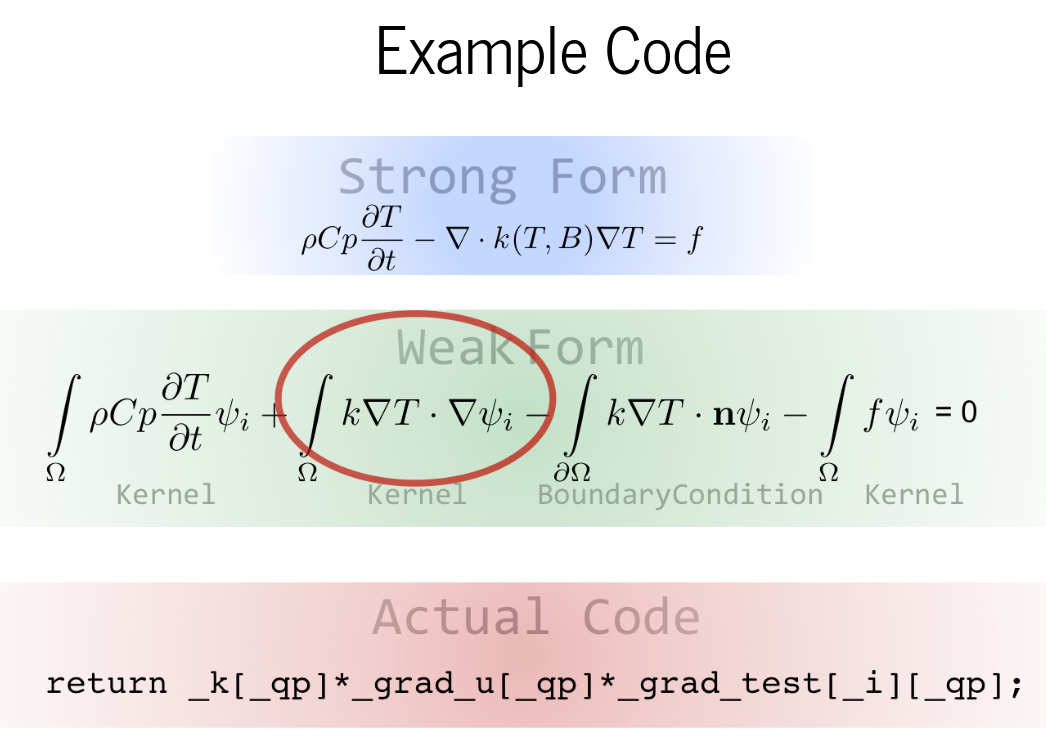
\includegraphics[width=8cm]{moose2}
    \end{center}
    \caption{Translation into MOOSE kernels procedure \cite{inl_workshop_2020}.}
\end{figure}
\end{frame}


\begin{frame}
\frametitle{Weak form: Equation 1}

\begin{align}
    & \left< D_{0,g} \nabla \Phi_{0,g}, \nabla \Psi \right> - \left< D_{0,g} \nabla \Phi_{0,g}, \Psi \right>_{BC} + \left< \Sigma_{0,g} \Phi_{0,g}, \Psi \right> + \left< - 2 \Sigma_{0,g} \Phi_{2,g}, \Psi \right> \notag \\ &+ \left< - \sum_{g'\ne g}^G \Sigma_{s0,g' \rightarrow g} \left( \Phi_{0,g'} - 2 \Phi_{2,g'} \right), \Psi \right> \notag \\ &+ \left< - \frac{\chi_g}{k_{eff}} \sum_{g'=1}^G \nu\Sigma_{f,g'} \left( \Phi_{0,g'} - 2 \Phi_{2,g'} \right), \Psi \right> + \left< - Q_{0,g}, \Psi \right> = 0 \label{eq:SP3-0g}
    \intertext{with the boundary condition}
    & \left< D_{0,g} \nabla \Phi_{0,g}, \Psi \right>_{BC} = \left< \frac{1}{2} \Phi_{0,g} - \frac{3}{4} \Phi_{2,g}, \Psi \right>_{BC}.
\end{align}
\end{frame}

\begin{frame}
\frametitle{Weak form: Equation 2}

\begin{align}
    & \left< D_{2,g} \nabla \Phi_{2,g}, \nabla \Psi \right> - \left< D_{2,g} \nabla \Phi_{2,g}, \Psi \right>_{BC} + \left< \left( \Sigma_{2,g} + \frac{4}{5} \Sigma_{0,g} \right) \Phi_{2,g}, \Psi \right> \notag \\ &+ \left< - \frac{2}{5} \Sigma_{0,g} \Phi_{0,g}, \Psi \right> + \left< \frac{2}{5} \sum_{g'\ne g}^G \Sigma_{s0,g' \rightarrow g} \left( \Phi_{0,g'} - 2 \Phi_{2,g'} \right), \Psi \right> \notag \\ &+ \left< \frac{2}{5} \frac{\chi_g}{k_{eff}} \sum_{g'=1}^G \nu\Sigma_{f,g'} \left( \Phi_{0,g'} - 2 \Phi_{2,g'} \right), \Psi \right> + \left< \frac{2}{5} Q_{0,g}, \Psi \right> = 0. \label{eq:SP3-2g}
    \intertext{with the boundary condition}
    & \left< D_{2,g} \nabla \Phi_{2,g}, \Psi \right>_{BC} = \left< -\frac{3}{40} \Phi_{0,g} + \frac{21}{40} \Phi_{2,g}, \Psi \right>_{BC}.
\end{align}
\end{frame}


\subsection{Kernels}
\begin{frame}
\frametitle{SP3 Kernels: Equation 1}

\begin{table}[htbp!]
  \centering
  \caption{$SP_3$ kernels.}
  \begin{tabular}{lc}
  \toprule
  Kernel                & Equation 1 \\
  \midrule
  P3Diffusion           & $\left< D_{0,g} \nabla \Phi_{0,g}, \nabla \Psi \right>$ \\
  P3SigmaR              & $\left< \Sigma_{0,g} \Phi_{0,g}, \Psi \right>$ \\
  P3SigmaCoupled        & $\left< - 2 \Sigma_{0,g} \Phi_{2,g}, \Psi \right>$ \\
  P3InScatter           & $\left< - \sum_{g'\ne g}^G \Sigma_{s0,g' \rightarrow g} \left( \Phi_{0,g'} - 2 \Phi_{2,g'} \right), \Psi \right>$ \\
  P3FissionEigenKernel  & $\left< - \frac{\chi_g}{k_{eff}} \sum_{g'=1}^G \nu\Sigma_{f,g'} \left( \Phi_{0,g'} - 2 \Phi_{2,g'} \right), \Psi \right>$ \\
  BodyForce             & $\left< - Q_{0,g}, \Psi \right>$ \\
  \midrule
  BC Kernel & \\
  \midrule
  Vacuum          & $\left< \frac{1}{2} \Phi_{0,g} - \frac{3}{4} \Phi_{2,g}, \Psi \right>_{BC}$ \\
  \bottomrule
  \end{tabular}
  \label{tab:kernels}
\end{table}
\end{frame}


\begin{frame}
\frametitle{SP3 Kernels: Equation 2}

\begin{table}[htbp!]
  \centering
  \caption{$SP_3$ kernels.}
  \begin{tabular}{lc}
  \toprule
  Kernel                & Equation 2 \\
  \midrule
  P3Diffusion           & $\left< D_{2,g} \nabla \Phi_{2,g}, \nabla \Psi \right>$ \\
  P3SigmaR              & $\left< \left( \Sigma_{2,g} + \frac{4}{5} \Sigma_{0,g} \right) \Phi_{2,g}, \Psi \right>$ \\
  P3SigmaCoupled        & $\left< - \frac{2}{5} \Sigma_{0,g} \Phi_{0,g}, \Psi \right>$ \\
  P3InScatter           & $\left< \frac{2}{5} \sum_{g'\ne g}^G \Sigma_{s0,g' \rightarrow g} \left( \Phi_{0,g'} - 2 \Phi_{2,g'} \right), \Psi \right>$ \\
  P3FissionEigenKernel  & $\left< \frac{2}{5} \frac{\chi_g}{k_{eff}} \sum_{g'=1}^G \nu\Sigma_{f,g'} \left( \Phi_{0,g'} - 2 \Phi_{2,g'} \right), \Psi \right>$ \\
  BodyForce             & $\left< \frac{2}{5} Q_{0,g}, \Psi \right>$ \\
  \midrule
  BC Kernel & \\
  \midrule
  Vacuum                & $\left< - \frac{3}{40} \Phi_{0,g} + \frac{21}{40} \Phi_{2,g}, \Psi \right>_{BC}$ \\
  \bottomrule
  \end{tabular}
  \label{tab:kernels}
\end{table}
\end{frame}


\subsection{Diffusion solver}
\begin{frame}
\frametitle{Moltres}

\begin{align}
  & \nabla \cdot D_g \nabla \phi_g - \Sigma_g^r \phi_g + \sum_{g' \ne g}^G \Sigma_{g'\rightarrow g}^s \phi_{g'} +
  \chi_g^t \sum_{g' = 1}^G \frac{1}{k_{eff}}\nu \Sigma_{g'}^f \phi_{g'} + Q_g = 0. \label{eq:diffusion-eig}
\end{align}
\end{frame}


\subsection{C5 MOX Benchmark}
\begin{frame}
\frametitle{Benchmark definition}

\begin{columns}
    \column[t]{4cm}
    \begin{itemize}
        \item 7-group cross-sections: C5G7 \cite{oecdnea_benchmark_2003}.
        \item Capilla et al \cite{capilla_applications_2009}: C5G2.
    \end{itemize}

    \column[t]{6cm}
    \begin{figure}[htbp!]
        \begin{center}
            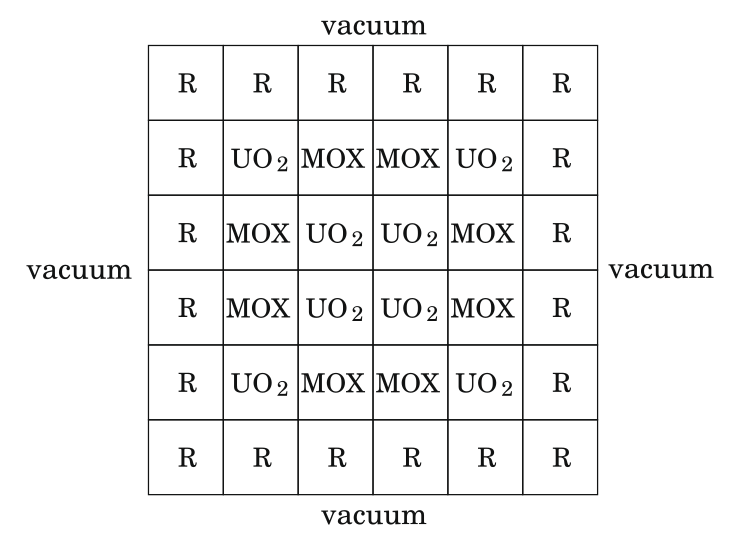
\includegraphics[width=6cm]{../C5G2-benchmark/bench-config}
        \end{center}
        \caption{2-D C5 MOX benchmark configuration. Image reproduced from \cite{capilla_applications_2009}. $R$ represents the reflectors.}
    \end{figure}
\end{columns}
\end{frame}


\begin{frame}
\frametitle{Benchmark definition (2)}

\begin{columns}
    \column[t]{5.5cm}
    \begin{figure}[htbp!]
        \begin{center}
            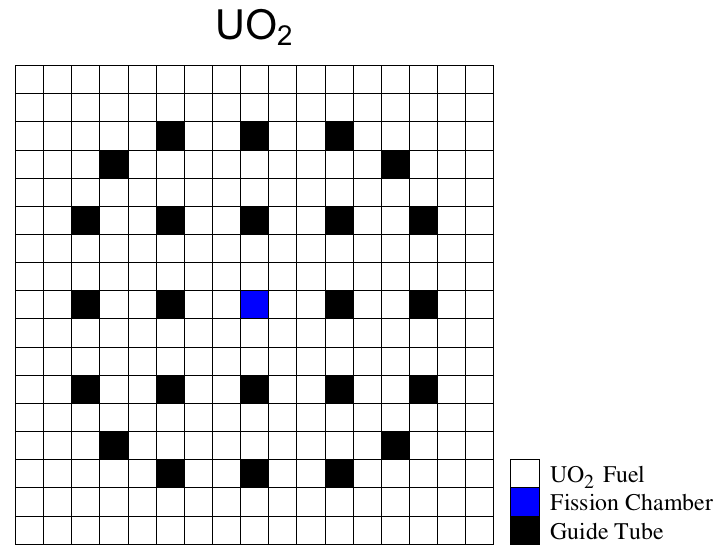
\includegraphics[width=5.5cm]{../C5G2-benchmark/bench-config2}
        \end{center}
        \caption{UO$_2$ assembly. Image reproduced from \cite{capilla_applications_2009}.}
    \end{figure}

    \column[t]{5.5cm}
    \begin{figure}[htbp!]
        \begin{center}
            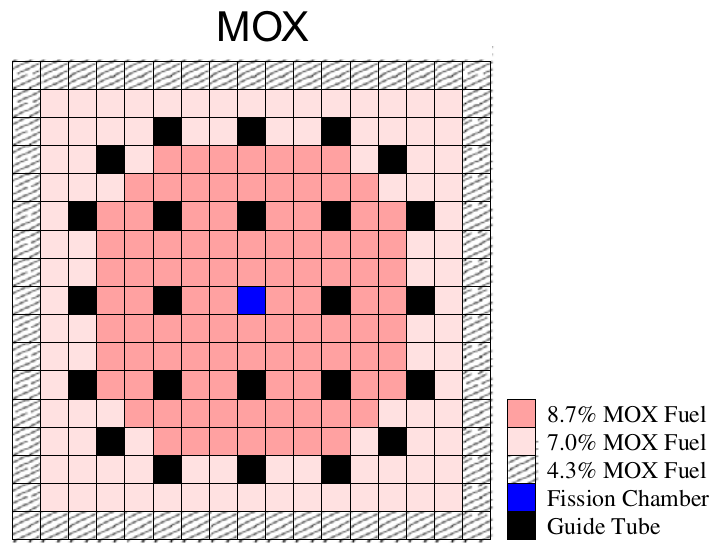
\includegraphics[width=5.5cm]{../C5G2-benchmark/bench-config3}
        \end{center}
        \caption{MOX assembly. Image reproduced from \cite{capilla_applications_2009}.}
    \end{figure}
\end{columns}
\end{frame}


\begin{frame}
\frametitle{Benchmark geometry}

    \begin{figure}[htbp!]
        \begin{center}
            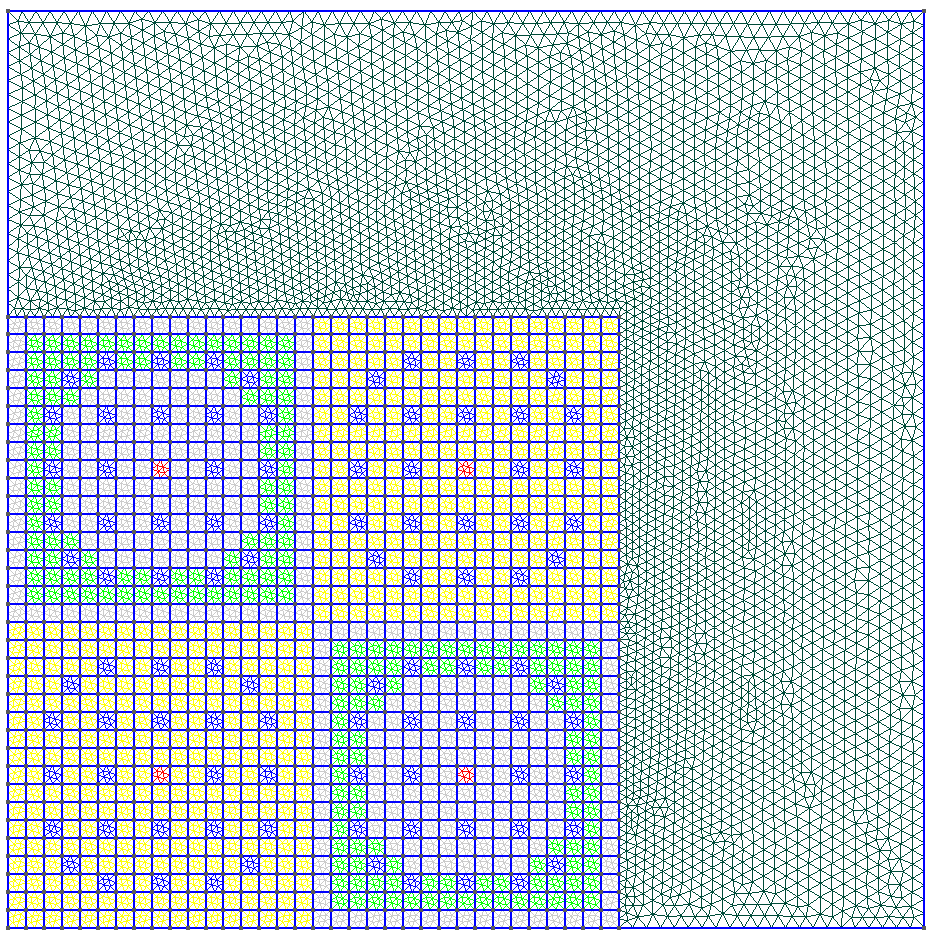
\includegraphics[width=6.cm]{bench-mesh}
        \end{center}
        \caption{Gmsh 2D geometry.}
    \end{figure}

\end{frame}
